% Interesting trick to instead make the chapter number the letter B for this appendix.
\begingroup
\renewcommand\thechapter{B}
\titleformat{\chapter}[display]
{\normalfont\huge\bfseries}{}{20pt}{\Huge}
\setcounter{section}{0} % Set the section counter back to 0 so Appendix A doesn't interfere.
\setcounter{figure}{0} % Set the figure counter back to 0 so Appendix A doesn't interfere.

\chapter*{Appendix B - Classification Algorithms}
\addcontentsline{toc}{chapter}{Appendix B - Classification Algorithms}
\markboth{Appendix B}{}

\section{Random Forest}
Random forests are ensemble models, meaning that they leverage multiple other models and average their findings to 
give a single result. The other models used by a random forest are decision trees, which are flowchart-like structures where 
data is split at each node of the tree based on feature values to arrive at a classification. Random forests create many decision 
trees based on randomly sampling the dataset, and these trees then classify rows based on what they learn. Then, the predictions 
for each row by all decision trees are aggregated, and the prediction reached by the most trees is used.
The amount of decision trees used is a parameter that can be set, and the computational requirements of the algorithm 
also increase alongside this amount.
% This was written half-asleep at 12am and likely doesn't make much sense.

\para Random forests are reputed as one of the best classification algorithms, and are used frequently in many fields 
including diabetes diagnosis as seen in works from \textcite{chang_pima_2023} and \textcite{alzubi_diabetes_2023},
demonstrating their suitability for this classification task.
% They're resistant to overfitting, too. Talk about this.

\section{Support Vector Machine}
Support vector machines aim to find the optimal hyperplane\footnote{A decision boundary that separates the classes. In a two-dimensional graph, this would be a line of best fit, but in a multidimensional dataset, it would be a hyperplane.}
which separates classes with the highest possible margin, and are commonly used in classification problems \autocite{ibm_what_2023}. Data points on either 
side of the margin are known as support vectors. Figure \ref{fig:OptimalSVM} shows how a perfect SVM would look in a two-dimensional dataset for demonstrative purposes.

\begin{figure}[H]
    \centering
    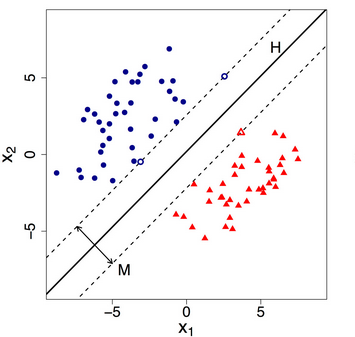
\includegraphics[width=.5\linewidth]{Algorithms/OptimalSVM.png}
    \caption{An optimal SVM that demonstrates the algorithm's key features. Rows on the dotted line are the support vectors, the solid line is the hyperplane, and the space
    between the hyperplane and support vectors is the margin. \autocite{kirchner_using_2018}}
    \label{fig:OptimalSVM}
\end{figure}

\para \textcite{kirchner_using_2018} state that SVMs are computationally intensive, requiring lots of memory and processing power 
to run optimally. Additionally, \textcite{atla_sensitivity_2011} mention that SVMs are particularly sensitive to noise in 
datasets, meaning their quality can be poor when there are many outliers. Despite these drawbacks, however, they can still 
be useful in diabetes classification as observed in the work of \textcite{zou_construction_2024}.

\section{Logistic Regression}
Logistic regression computes a weighted sum of all input features, where the appropriate weights are learned by the algorithm as it trains.
A sigmoid function, shown in Equation \ref{eq:Sigmoid}, is then used to transform the sum to a value between 0 and 1, which is then used to classify the row as 0 if it is below 
0.5, or classify it as 1 if it is above 0.5. 

\begin{equation}\label{eq:Sigmoid}
    f(x) = \frac{1}{1 + e^{-x}}     
\end{equation}

\para Logistic regression is a very common algorithm in binary classification tasks, as it is simple to implement and interpret, and
can perform well even with limited amounts of training data \autocite{kavya_applications_2024}. It has also been widely used in previous 
analyses of the Pima Indian dataset. (\textcite{alzubi_diabetes_2023}, \textcite{joshi_predicting_2021}, \textcite{zou_construction_2024})

\section{Na\"ive Bayes}
Na\"ive Bayes is an example of a probabilistic classification algorithm \autocite{ibm_what_2021}, as it is based on Bayes' theorem,
which calculates the probability of an event given that another event has occurred, shown in Equation \ref{eq:Bayes}. 
In binary classification, it is the probability of the target given the other features. Na\"ive Bayes gets its name from its na\"ive assumption
that features are all independent of each other.

\begin{equation}\label{eq:Bayes}
    P(A|B) = \frac{P(B|A) \cdot P(A)}{P(B)}
\end{equation}

\para This theorem calculates that the probability of an event occurring is equal to the probability of the event given 
prior knowledge multiplied by the prior probability of the event. This can be contextualised to this specific dataset, shown in Equation \ref{eq:ContextBayes}.

\begin{equation}\label{eq:ContextBayes}
    P(Diabetes | Other features) = \frac{P(Other features | Diabetes) \cdot P(Diabetes)}{P(Other features)}
\end{equation}

\para Gaussian Na\"ive Bayes is used in this project, as it is best suited to continuous data as seen in this dataset's 
features. Interestingly, Na\"ive Bayes typically has lower accuracy than other models such as Random Forests \autocite{khan_novel_2023},
though it has been used in previous diabetes classification tasks \autocite{aftab_cloud-based_2021, chang_pima_2023, zou_construction_2024}.

\section{K-Nearest Neighbours (KNN)}
The K-Nearest Neighbours (KNN) algorithm is a fundamental machine learning classification method that operates by identifying 
the $k$ closest training examples to a data point across all features and assigns the most common class among these neighbours 
as the prediction. $K$ is a parameter that can be set within the algorithm, and has a heavy influence over its accuracy.
KNN doesn't make any assumptions about the distribution of the data, making it useful for complex, real-world scenarios
such as healthcare \autocite{thomas_addressing_2021}, and has also been used on the Pima Indian and Frankfurt datasets
to high success \autocite{alzubi_diabetes_2023, zou_construction_2024}.

